\subsection{Задача 2: поиск глобального минимума}

\subsubsection{функция с одним глобальным минимумом}

\begin{figure}[H]
		\centering
			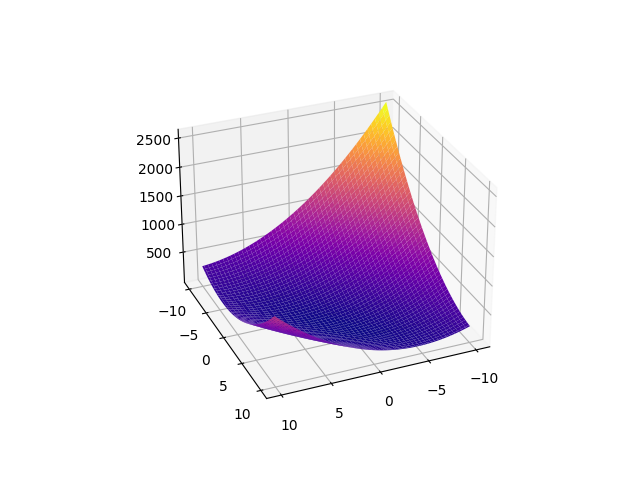
\includegraphics{task2/resources/Figure_1.png}
		\caption{График функции Бута}
		\label{w_pert}
	\end{figure}

Рассматриваемая функция Бута $f(x, y)$ имеет один глобальный минимум. Заранее известны точка минимума и значение функции в ней:

\begin{table}[H]
	\centering
	\begin{tabular}{| c | c | c |}
		\hline
		    x_{min} & y_{min} & f(x_{min}, y_{min}) \\
		\hline
		    1 & 3 & 0 \\
   		\hline
	\end{tabular}
	\caption{Все точки минимумов функции Бута и их значения}
\end{table}

Рассмотрим работу алгоритма поиска глобального минимума на начальном брусе \textbf{A} = [(-10, 10), (-10, 10)], $\epsilon = 0.01$. Черная линия - путь работы алгоритма, красная точка - найденный алгоритмом глобальный минимум.

\begin{figure}[H]
	\centering
		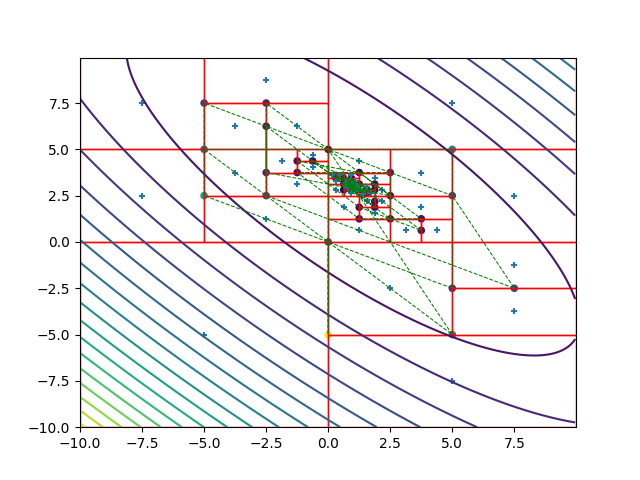
\includegraphics{task2/resources/Figure_2.png}
	\caption{Поиск глобального минимума функции Бута}
	\label{w_pert}
\end{figure}

\begin{table}[H]
	\centering
	\begin{tabular}{| c | c | c |}
		\hline
		    x* & y* & f(x*, y*) \\
		\hline
		    1.025390625 & 2.98828125 & 0 \\
   		\hline
	\end{tabular}
	\caption{Найденный алгоритмом глобальный минимум функции Бута}
\end{table}

\newpage
\subsubsection{Функция с несколькими глобальными минимумами}

\begin{figure}[H]
		\centering
			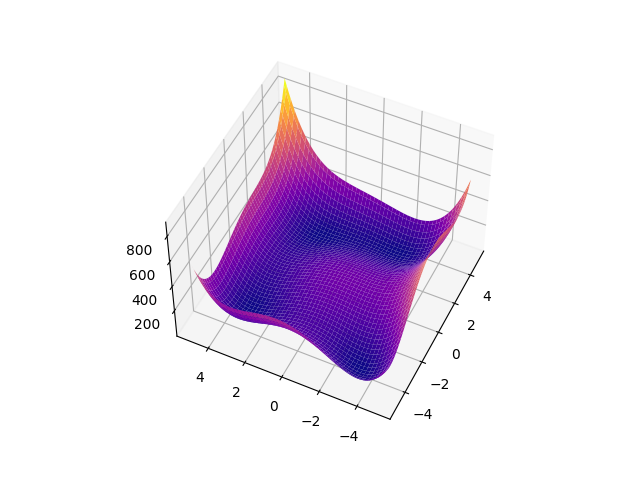
\includegraphics{task2/resources/Figure_3.png}
		\caption{График функции Химмельблау}
		\label{w_pert}
	\end{figure}

Рассматриваемая функция Химмельблау $f(x, y)$ имеет четыре глобальных минимума. Заранее известны точки минимумы и значения функций в ней:

\begin{table}[H]
	\centering
	\begin{tabular}{| c | c | c |}
		\hline
		    x_{min} & y_{min} & f(x_{min}, y_{min}) \\
		\hline
		    3 & 2 & 0 \\
		    -2.805118 & 3.131312 & 0 \\
		    -3.779310 & -3.283186 & 0 \\
		    3.584428 & -1.848126 & 0 \\
   		\hline
	\end{tabular}
	\caption{Все точки минимумов функции Химмельблау и их значения}
\end{table}

Рассмотрим работу алгоритма поиска глобального минимума на начальном брусе \textbf{A} = [(-5, 5), (-5, 5)], $\epsilon = 0.01$. Черная линия - путь работы алгоритма, красная точка - найденный алгоритмом глобальный минимум.

\begin{figure}[H]
	\centering
		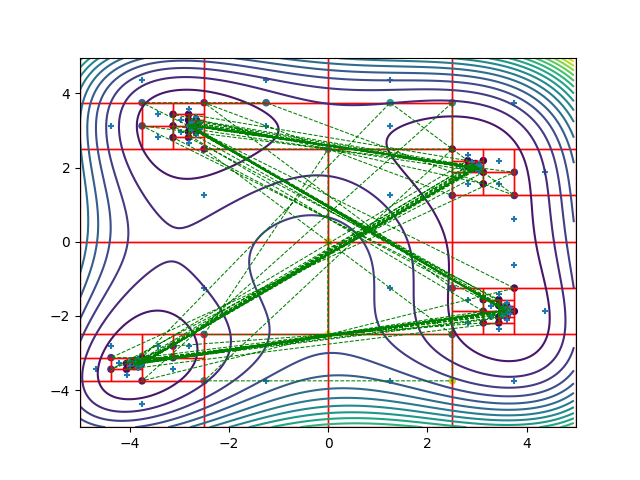
\includegraphics{task2/resources/Figure_4.png}
	\caption{Поиск глобального минимума функции Химмельблау}
	\label{w_pert}
\end{figure}

\begin{table}[H]
	\centering
	\begin{tabular}{| c | c | c |}
		\hline
		    x* & y* & f(x*, y*) \\
		\hline
		    2.998046875 & 2.001953125 & 0 \\
   		\hline
	\end{tabular}
	\caption{Найденный алгоритмом глобальный минимум функции Химмельблау}
\end{table}
